\documentclass[11pt,a4paper]{article}
\usepackage[utf8]{inputenc}
\usepackage[spanish]{babel}
\usepackage{amsmath}
\usepackage{amsfonts}
\usepackage{amssymb}
\usepackage{makeidx}
\usepackage{graphicx}
\usepackage{lmodern}
\usepackage{kpfonts}
\usepackage[left=2cm,right=2cm,top=2cm,bottom=2cm]{geometry}
\author{Miguel Angel Xamie Diaz Fuentes}
\usepackage{apacite}

\begin{document}
\begin{center}
\begin{LARGE}
\textbf{INGENIERÍA MECATRÓNICA}\\
\end{LARGE}
Sistemas Eletrónicos De Interfaz\\
\begin{figure}[hbtp]
\centering

\includegraphics[scale=0.70]{UPZMG_Mecatr_nica.png}
\end{figure} 
\begin{center}
{\Large \emph{EV-1-6 EXPLICAR LA OPERACIÓN DE LOS CIRCUITOS DE ACTIVACION CON TIRISTORES EN CONVERTIDORES CA-CD Y CA-CA}}
\end{center}

\textbf{Alumno}
\\\textit{Miguel Angel Xamie Diaz Fuentes}
\textbf{\\Maestro}
\\\textit{Morán Garabito Carlos Enriquez}
\textbf{\\Fecha de Entrega}
\\\textit{24/09/2019}
\textbf{\\Grupo}
\\\textit{4-B}
\end{center}

\footnote{Universidad Politécnica De La Zona Metropolitana De Guadalajara} 

\pagebreak

\section{Explicar la operación de los circuitos de activación con tiristores en convertidores CA-CD y CA-CA}
\subsection{En convertidores CA-CD}

Para este rectificador de onda completa cuya carga puede ser puramente resistiva. El convertidor CA-CD nos proporciona una señal de salida rectificada (casi constante) de valor Vm, donde Vm es igual al valor pico del voltaje de entrada.\\
En los circuitos rectificadores se puede sustituir total o parcial a los diodos por tiristores, obteniendo un sistema de rectificación controlado (formados únicamente por tiristores) o semicontrolados (formado por tiristores o diodos).\\
La puerta es la encargada de controlar el paso de corriente entre el ánodo y el cátodo. Funciona básicamente como un diodo rectificador controlado, permitiendo circular la corriente en un solo sentido.\\
\textbf{Para la activación} cuando le llega una pequeña corriente a la puerta G, se activa el tiristor (interruptor cerrado entre ánodo y cátodo) y comenzará a pasar una corriente entre el ánodo y el cátodo llamada corriente directa. Mientras no le llegue corriente a la puerta G no habrá corriente entre el ánodo y el cátodo (interruptor abierto). El interruptor es el ánodo y el cátodo; y la puerta G es la que lo cierra o lo abre (activación) por medio de una señal eléctrica.\\

\textbf{Para la desactivación} una vez que el tiristor se activa, permanece activado (interruptor cerrado) aunque cortemos la corriente por la patilla o puerta G. En el transistor cuando le deja de llegar corriente a la base se desactiva. Si queremos que deje de pasar corriente entre el ánodo y el cátodo del tiristor la única forma es desconectando la corriente directa de alguna manera como luego veremos.\\

Con un transistor, cuando una pequeña corriente fluye en la base, hace que un flujo de corriente más grande se genere entre el emisor y el colector. En otras palabras, que actúa como un interruptor y un amplificador al mismo tiempo.

\begin{figure}[hbtp]
\centering
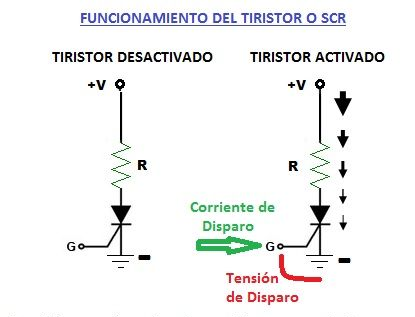
\includegraphics[scale=0.70]{ACTIVACION.png}
\end{figure} 
\begin{figure}[hbtp]
\centering
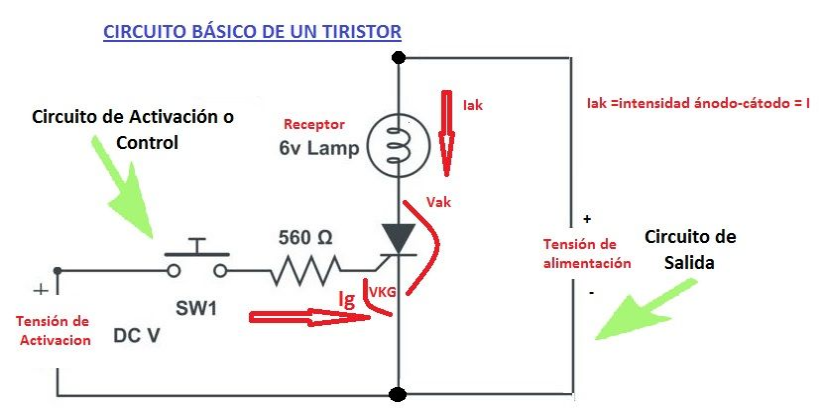
\includegraphics[scale=0.40]{ca-cd.png}
\end{figure}

\footnote{Universidad Politécnica De La Zona Metropolitana De Guadalajara} 
 
\pagebreak

Una vez que el tiristor se activa y pasa corriente por la lámpara (entre ánodo y cátodo); la señal de la puerta G pierde todo el control debido a la acción de enganche de los dos transistores internos (que forman el ánodo y cátodo), es decir se auto-bloquea. Por eso decíamos que una vez activado da igual si deja de pasar corriente por G, la corriente de salida I seguirá circulando por el circuito de salida. De hecho si te fijas en el esquema para activar la puerta hemos puesto un pulsador, al apretarlo se activa y al soltarlo deja de pasar corriente a G.\\

 La aplicación de corriente por la puerta momentáneamente, es suficiente para hacer que se realice y se mantenga de forma permanente (ON) incluso si la señal de puerta se elimina por completo. Para desactivarlo tenemos que cortar la corriente en el circuito de salida, es decir que deje de tener corriente entre el ánodo y el cátodo (desconectarlos). Por es motivo se suele poner un interruptor también en el circuito de salida. También es cierto que hay una corriente de ánodo por debajo de la cual el tiristor deja de estar activa sin llegar esta a 0V, esta corriente se llama "corriente de mantenimiento" (IH).
 
 
 
 
 
 
\subsection{En convertidores CA-CA}
el tiristor debe siempre estar polarizado directamente, es decir el ánodo al positivo y el cátodo al negativo, para que pueda empezar a pasar la corriente entre ellos al activarlo, ya que es en el sentido que deja circular corriente entre ánodo y cátodo. Si está polarizado indirectamente nunca pasará corriente entre el ánodo y el cátodo aunque tengamos corriente en la puerta G.\\

 La corriente necesaria (o mínima) que le tiene que llegar a G para activar el tiristor es lo que se conoce como "Corriente de Disparo". Podríamos hablar de la tensión a la que se activa, en lugar de corriente (ya sabes que para que exista corriente necesitamos una tensión), en este caso se llamará "Tensión de Disparo".\\

 Otra característica del tiristor es que la tensión o corriente de disparo no es fija, a mayor corriente de disparo (corriente por G = Ig) menor será la tensión de disparo o ruptura Vr. Fíjate en la gráfica siguiente:\\
 
\begin{figure}[hbtp]
\centering
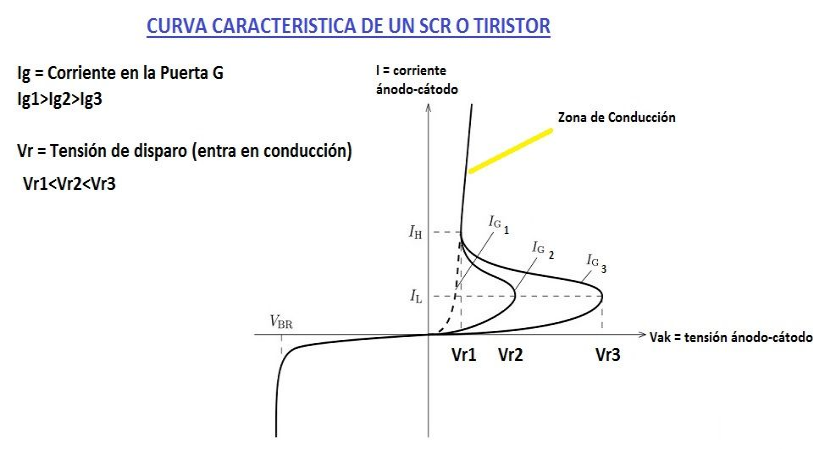
\includegraphics[scale=0.40]{DATOS.png}
\end{figure} 

Para un tiristor polarizado directamente, la inyección de una corriente por la puerta G al aplicar una tensión positiva entre la puerta G y el cátodo (K) lo activará. Si aumentamos la corriente en G disminuirá la tensión de disparo del tiristor. Fíjate en el siguiente circuito básico con las corrientes y las tensiones.\\

\footnote{Universidad Politécnica De La Zona Metropolitana De Guadalajara} 

\pagebreak

La mayoría de las aplicaciones de los tiristores o/y los SCR son para controlar un circuito de alimentación o salida en corriente alterna (interruptor). Como ya dijimos, el tiristor solo conduce si está polarizado directamente, es decir si el ánodo está al polo positivo y el cátodo al negativo.

\footnote{Universidad Politécnica De La Zona Metropolitana De Guadalajara} 

\begin{figure}[hbtp]
\centering
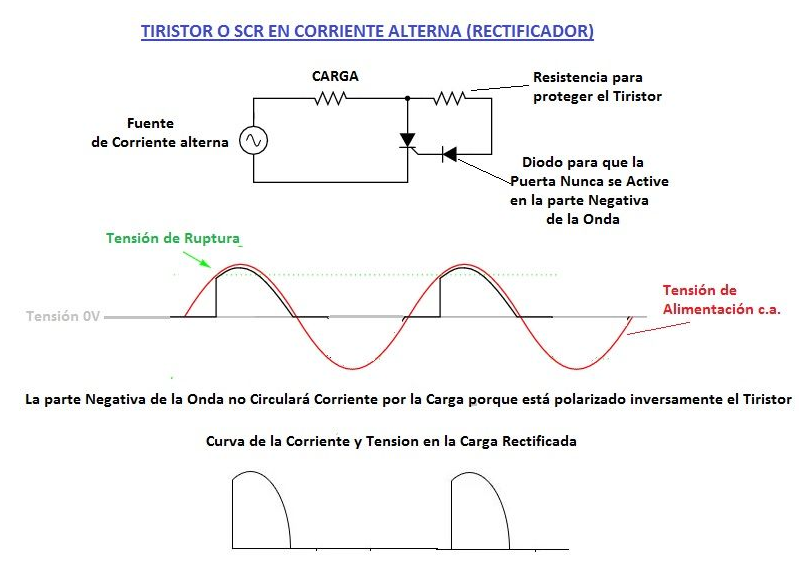
\includegraphics[scale=0.40]{ca-ca.png}
\end{figure} 

Durante el semiciclo positivo de la fuente de corriente alterna (c.a.) el ánodo del tiristor o SCR es mas positivo que el cátodo y están polarizados directamente. Si ahora le llega una señal suficiente a la puerta el tiristor se activará y pasará corriente de entre ánodo y cátodo. Al principio del ciclo positivo de la onda como no le llega la suficiente corriente a la puerta el tiristor estará desactivado. Llegará un momento que le llegue la suficiente corriente o tensión (tensión de disparo) y es entonces cuando el tiristor se activará. Una parte de la onda no estará en la salida al principio.\\


Al pasar por cero, mejor dicho por el valor de la corriente de mantenimiento IK, el tiristor se desconecta (sin corriente de salida = interruptor abierto). Durante el otro medio ciclo la polaridad de la fuente es negativa, y esta polaridad hace que el tiristor o SCR quede inversamente polarizado lo cual impide que circule cualquier corriente hacia la carga. Esto significa que no puede estar en conducción por más de medio ciclo. Al volver al ciclo positivo necesitamos activar de nuevo el tiristor con una pequeña corriente en la puerta, pero como está conectada también a la fuente de tensión en alterna, la propia fuente nos la genera.\\
Pues resulta que en la parte de la onda positiva de corriente alterna circula corriente y por la parte negativa no circula corriente, haciendo el tiristor de rectificador, ya que la onda de salida quedaría rectificada (solo la parte positiva).


\footnote{Universidad Politécnica De La Zona Metropolitana De Guadalajara} 

\pagebreak

\begin{thebibliography}
 \\Referencias URL
\end{thebibliography}
\begin{flushleft}
\url{https://www.areatecnologia.com/electronica/tiristor.html}\\
\url{https://prezi.com/dh380hlerc-l/convertidores-ca-cd
/?fbclid=IwAR0Gfiz-T0OoXSgGnGF95TXffk8MrBAAWTbQ6ZueAlAjTIsF15C-YD1vpDQ }\\
\url{http://ccpot.galeon.com/enlaces1737112.html }\\
\url{https://www.monografias.com/trabajos105/convertidores-
ca-cc-y-ca-ca-tiristores/convertidores-ca-cc-y-ca-ca-tiristores.shtml?fbclid=IwAR3QDEmykUhgtxBc-hwdGgGqBIZUenI6WL42IQz9DXZho978FnHeNXTT0oE}
\end{flushleft}





\end{document}
